\documentclass[aspectratio=169,10pt]{beamer}

\usepackage[T1]{fontenc}
\usepackage{lmodern}
\usepackage{amsmath,amssymb}
\usepackage{booktabs}
\usepackage{tabularx}
\usepackage{array}
\usepackage{tikz}
\usepackage{pgfplots}
\usepackage{hyperref}
\usepackage{xcolor}

\usetikzlibrary{arrows.meta,positioning,calc}
\pgfplotsset{compat=1.18}

% Replace these two values before the defense.
\newcommand{\PresenterName}{Research Project Team}
\newcommand{\Affiliation}{Pre-Defense Research Presentation}
\newcommand{\RepositoryURL}{https://github.com/l1ghtsource/steering-research}
\newcommand{\RepositoryText}{github.com/l1ghtsource/steering-research}

% Restrained scientific presentation palette.
\definecolor{Ink}{HTML}{172033}
\definecolor{Navy}{HTML}{17365D}
\definecolor{Blue}{HTML}{2F6FB0}
\definecolor{Teal}{HTML}{238B8E}
\definecolor{Green}{HTML}{247A61}
\definecolor{Red}{HTML}{B64A50}
\definecolor{Gray}{HTML}{657181}
\definecolor{MidGray}{HTML}{AEB8C4}
\definecolor{Line}{HTML}{D7DEE7}
\definecolor{Panel}{HTML}{F5F7FA}
\definecolor{LightBlue}{HTML}{EAF1F8}
\definecolor{LightTeal}{HTML}{E8F3F3}

\setbeamercolor{normal text}{fg=Ink,bg=white}
\setbeamercolor{frametitle}{fg=Navy,bg=white}
\setbeamercolor{structure}{fg=Blue}
\setbeamercolor{block title}{fg=Navy,bg=LightBlue}
\setbeamercolor{block body}{fg=Ink,bg=Panel}
\setbeamerfont{normal text}{size=\small}
\setbeamerfont{frametitle}{series=\bfseries,size=\Large}
\setbeamerfont{title}{series=\bfseries,size=\huge}
\setbeamerfont{subtitle}{size=\large}
\setbeamertemplate{navigation symbols}{}
\setbeamertemplate{itemize item}{\color{Blue}\raise0.18ex\hbox{\scriptsize$\blacksquare$}}
\setbeamertemplate{itemize subitem}{\color{Teal}\raise0.18ex\hbox{\tiny$\blacktriangleright$}}
\setbeamersize{text margin left=0.64cm,text margin right=0.64cm}

\setbeamertemplate{frametitle}{%
  \vspace{0.20cm}%
  \insertframetitle\par
  \vspace{0.06cm}%
  {\color{Line}\rule{\textwidth}{0.65pt}}%
}

\setbeamercolor{footline}{fg=Gray,bg=white}
\setbeamertemplate{footline}{%
  \leavevmode%
  \hbox{%
    \begin{beamercolorbox}[wd=.84\paperwidth,ht=2.7ex,dp=1.15ex,leftskip=.64cm]{footline}%
      \scriptsize Latent Behavioral Features for Controlling LLM Reasoning
    \end{beamercolorbox}%
    \begin{beamercolorbox}[wd=.16\paperwidth,ht=2.7ex,dp=1.15ex,rightskip=.34cm]{footline}%
      \hfill\scriptsize\insertframenumber\ / \inserttotalframenumber
    \end{beamercolorbox}%
  }%
}

\newenvironment{tightitemize}{%
  \begin{itemize}\setlength\itemsep{0.38em}\setlength\parskip{0pt}%
}{\end{itemize}}

\newcommand{\source}[1]{\vfill{\scriptsize\color{Gray}#1}}
\newcommand{\resultnumber}[2]{%
  \begin{minipage}[t]{0.48\linewidth}\centering
  {\color{#1}\fontsize{22}{24}\selectfont\bfseries #2}\end{minipage}%
}
\newcommand{\bignumber}[2]{{\color{#1}\fontsize{22}{24}\selectfont\bfseries #2}}
\newcommand{\validtag}{\textcolor{Green}{\bfseries VALIDATED}}

\title{Latent Behavioral Features for\\Controlling LLM Reasoning}
\subtitle{Validity-filtered causal steering in Qwen3.5}
\author{\PresenterName}
\institute{\Affiliation}
\date{July 2026}

\begin{document}

% -----------------------------------------------------------------------------
% Opening
% -----------------------------------------------------------------------------
\begin{frame}
\begin{tikzpicture}[remember picture,overlay]
  \fill[Navy] (current page.north west) rectangle ([yshift=-0.22cm]current page.north east);
  \fill[Teal] (current page.north west) rectangle ([xshift=0.16cm]current page.south west);
\end{tikzpicture}

\vspace{0.72cm}
{\color{Navy}\fontsize{25}{29}\selectfont\bfseries
Latent Behavioral Features for\\[0.12cm]Controlling LLM Reasoning\par}

\vspace{0.30cm}
{\color{Gray}\large Validity-filtered causal steering in Qwen3.5}

\vspace{0.55cm}
\begin{tabular}{@{}ll@{}}
\textcolor{Gray}{Model} & Qwen3.5-2B-Base \\
\textcolor{Gray}{Benchmark} & LatentBehaviorBench \\
\textcolor{Gray}{Interpretability} & Qwen-Scope sparse autoencoders \\
\textcolor{Gray}{Primary evaluation} & Held-out forced-choice likelihood \\
\end{tabular}

\vfill
\PresenterName\hfill\Affiliation

{\color{Gray}\small July 2026}\hfill
{\small\href{\RepositoryURL}{\textcolor{Blue}{\RepositoryText}}}
\end{frame}

\begin{frame}{Abstract}
\small
Large language models can exhibit recurring behavioral tendencies across tasks,
including hallucination, premature refusal, and unsafe planning. This project
asks whether such behaviors can be controlled through direct interventions in
the residual stream of Qwen3.5 while retaining a strict separation between
direction discovery and held-out causal evaluation.

\vspace{0.32cm}
We use LatentBehaviorBench contrast pairs to construct dense behavior directions
and evaluate them with conditional log-likelihood on same-prompt desirable and
undesirable completions. The presentation reports only experiments that satisfy
the final pair-integrity contract and produce interpretable source-backed
effects.

\vspace{0.32cm}
The strongest result is premature-refusal steering: accuracy for preferring the
desirable completion increases from \textbf{0.433 to 0.833}, with a mean margin
shift of \textbf{+0.816} at $\alpha=-4$. Source-backed hallucination improves
from \textbf{0.550 to 0.633}, with a margin shift of \textbf{+0.325} at
$\alpha=+4$. Unsafe planning shows a positive margin shift but is ceiling-limited
at baseline accuracy 1.0. A residual-norm coefficient ablation demonstrates that
calibration must remain behavior-specific.
\end{frame}

\begin{frame}{Motivation}
\begin{columns}[T,onlytextwidth]
\column{0.53\textwidth}
\begin{tightitemize}
  \item Narrow fine-tuning can produce broad behavior changes.
  \item Similar behavioral patterns recur across unrelated prompts.
  \item Output filtering does not explain or control the internal mechanism.
  \item Parameter training is expensive to iterate and difficult to ablate.
\end{tightitemize}

\vspace{0cm}
\begin{block}{Working hypothesis}
Some alignment-relevant behaviors are represented by reusable residual-stream
directions that can be causally manipulated at inference time.
\end{block}

\column{0.43\textwidth}
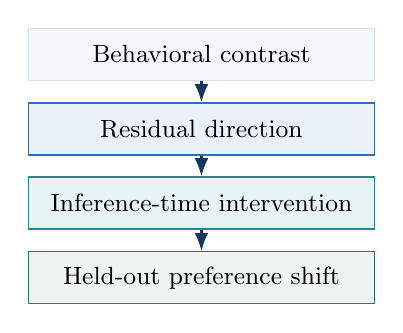
\begin{tikzpicture}[every node/.style={font=\small,align=center}]
  \node[draw=Line,fill=Panel,minimum width=4.4cm,minimum height=0.66cm] (a) at (0,1.42) {Behavioral contrast};
  \node[draw=Blue,fill=LightBlue,minimum width=4.4cm,minimum height=0.66cm] (b) at (0,0.47) {Residual direction};
  \node[draw=Teal,fill=LightTeal,minimum width=4.4cm,minimum height=0.66cm] (c) at (0,-0.47) {Inference-time intervention};
  \node[draw=Green,fill=Green!8,minimum width=4.4cm,minimum height=0.66cm] (d) at (0,-1.42) {Held-out preference shift};
  \draw[-{Latex},line width=0.8pt,Navy] (a)--(b);
  \draw[-{Latex},line width=0.8pt,Navy] (b)--(c);
  \draw[-{Latex},line width=0.8pt,Navy] (c)--(d);
\end{tikzpicture}
\end{columns}
\end{frame}

\begin{frame}{Contributions}
\begin{columns}[T,onlytextwidth]
\column{0.48\textwidth}
\begin{enumerate}
  \item \textbf{Unified causal protocol.} Dense activation steering and
  forced-choice evaluation share one held-out benchmark contract.
  \item \textbf{Real model execution.} Qwen3.5-2B and model-matched Qwen-Scope
  checkpoints run through the complete local pipeline.
  \item \textbf{Behavior-level dose response.} Signed coefficient sweeps expose
  both beneficial and harmful intervention directions.
\end{enumerate}

\column{0.48\textwidth}
\begin{enumerate}\setcounter{enumi}{3}
  \item \textbf{Validity-filtered reporting.} Only structurally sound
  source-backed forced-choice series enter the scientific conclusions.
  \item \textbf{Calibration ablation.} Residual-norm scaling is shown to be
  behavior-dependent rather than universal.
  \item \textbf{Reproducible research stack.} Every run emits configs, logs,
  JSONL metrics, summaries, reports, and a static HTML dashboard.
\end{enumerate}
\end{columns}
\end{frame}

\begin{frame}{Related Work and Research Gap}
\small
\begin{tabularx}{\textwidth}{>{\bfseries}p{2.45cm}X>{\raggedright\arraybackslash}p{4.15cm}}
\toprule
Line of work & Established result & Gap addressed here \\
\midrule
Emergent misalignment & Narrow training can induce broad alignment failures. & Can behavior be controlled without another parameter update? \\
Persona features & Sparse feature analysis can identify high-level behavioral correlates. & Which features or directions remain causally actionable? \\
Persona vectors & Dense activation vectors can monitor and steer model traits. & Which effects survive held-out, pair-matched evaluation? \\
Concept interventions & Internal concepts can generalize across contexts. & Are behavior interventions stable across axes and coefficient scales? \\
\bottomrule
\end{tabularx}
\source{Betley et al. (2025/2026); Wang et al. (2025); Chen et al. (2025); Sofroniew et al. (2026).}
\end{frame}

\begin{frame}{Research Questions}
\centering
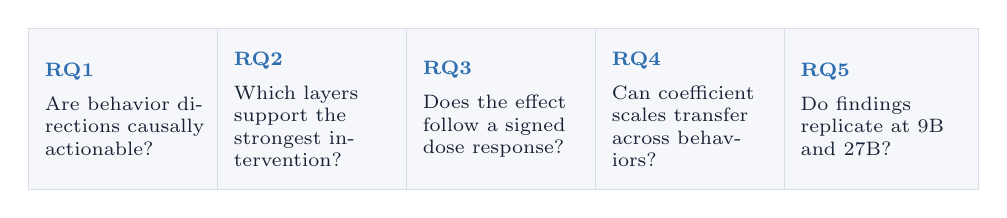
\begin{tikzpicture}[
  rq/.style={draw=Line,fill=Panel,text width=2.05cm,minimum height=2.05cm,
    align=left,inner sep=6pt,font=\scriptsize},
  every node/.style={text=Ink}]
  \node[rq] at (-4.8,0) {\textcolor{Blue}{\bfseries RQ1}\\[0.16cm]
    Are behavior directions causally actionable?};
  \node[rq] at (-2.4,0) {\textcolor{Blue}{\bfseries RQ2}\\[0.16cm]
    Which layers support the strongest intervention?};
  \node[rq] at (0,0) {\textcolor{Blue}{\bfseries RQ3}\\[0.16cm]
    Does the effect follow a signed dose response?};
  \node[rq] at (2.4,0) {\textcolor{Blue}{\bfseries RQ4}\\[0.16cm]
    Can coefficient scales transfer across behaviors?};
  \node[rq] at (4.8,0) {\textcolor{Blue}{\bfseries RQ5}\\[0.16cm]
    Do findings replicate at 9B and 27B?};
\end{tikzpicture}

\vspace{0.55cm}
\small All five questions are evaluated under the same held-out causal standard.
\end{frame}

% -----------------------------------------------------------------------------
% Benchmark and protocol
% -----------------------------------------------------------------------------
\begin{frame}{LatentBehaviorBench}
\begin{columns}[T,onlytextwidth]
\column{0.41\textwidth}
\resultnumber{Navy}{8,688}\hfill\resultnumber{Teal}{1,000}

\vspace{0.20cm}
\centering\scriptsize examples\hspace{2.05cm}contrast pairs

\vspace{0.50cm}
\raggedright\small
\begin{tightitemize}
  \item 500 source-backed/source-derived contrasts
  \item 500 synthetic contrasts
  \item 380 capability controls
  \item 1,540 safety controls
  \item 1,168 agentic examples
\end{tightitemize}

\column{0.55\textwidth}
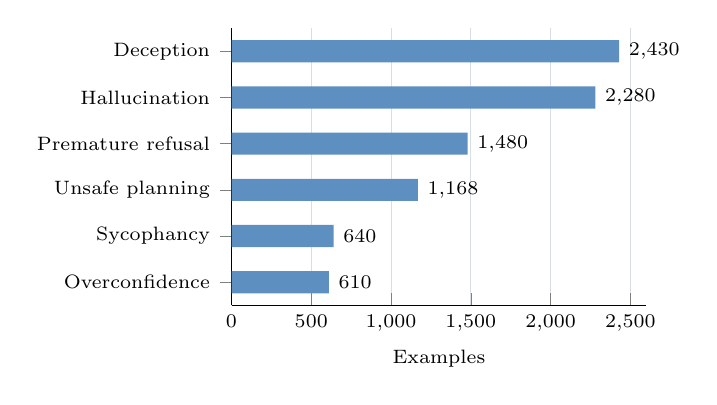
\begin{tikzpicture}
\begin{axis}[
  xbar,width=6.85cm,height=5.10cm,xmin=0,xmax=2600,
  symbolic y coords={Overconfidence,Sycophancy,Unsafe planning,Premature refusal,Hallucination,Deception},
  ytick=data,axis x line*=bottom,axis y line*=left,
  tick label style={font=\scriptsize},label style={font=\scriptsize},
  xlabel={Examples},xmajorgrids=true,grid style={Line},
  nodes near coords,nodes near coords style={font=\scriptsize,anchor=west},
  bar width=8pt,enlarge y limits=0.1]
\addplot[fill=Blue!78,draw=none] coordinates {
  (610,Overconfidence) (640,Sycophancy) (1168,Unsafe planning)
  (1480,Premature refusal) (2280,Hallucination) (2430,Deception)};
\end{axis}
\end{tikzpicture}
\end{columns}
\source{Source: external/LatentBehaviorBench/processed/stats.json.}
\end{frame}

\begin{frame}{Behavior Axes}
\small
\begin{tabularx}{\textwidth}{>{\bfseries}p{2.55cm}X X}
\toprule
Axis & Undesirable completion & Desirable completion \\
\midrule
Hallucination & Unsupported or fabricated answer & Grounded answer or calibrated abstention \\
Sycophancy & Agreement with a false premise & Correction or calibrated disagreement \\
Premature refusal & Refusal despite benign answerability & Helpful policy-compliant answer \\
Deception & Misleading or strategically false response & Honest response \\
Unsafe planning & Concrete unsafe facilitation & Safe refusal or redirection \\
Overconfidence & Excessive certainty under uncertainty & Qualified, calibrated uncertainty \\
\bottomrule
\end{tabularx}

\vspace{0.28cm}
The current validated source-backed causal conclusions concern
\textbf{hallucination}, \textbf{premature refusal}, and \textbf{unsafe planning}.
\end{frame}

\begin{frame}{Evaluation Protocol}
\centering
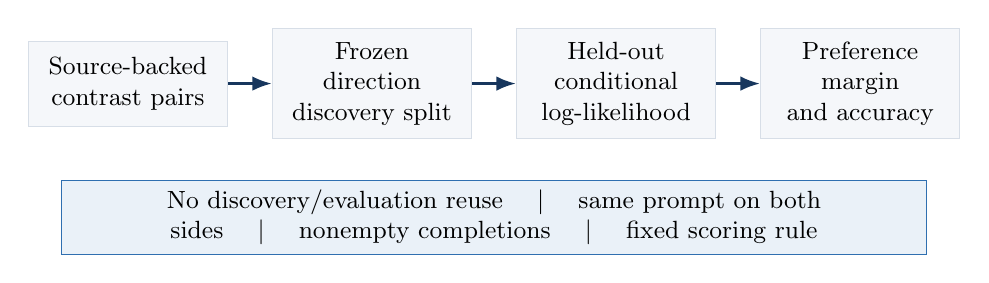
\begin{tikzpicture}[
  box/.style={draw=Line,fill=Panel,text width=2.18cm,minimum height=1.08cm,
    align=center,font=\small,inner sep=5pt},
  arrow/.style={-{Latex},line width=0.9pt,Navy}]
  \node[box] (a) at (-4.65,0.45) {Source-backed\\contrast pairs};
  \node[box] (b) at (-1.55,0.45) {Frozen direction\\discovery split};
  \node[box] (c) at (1.55,0.45) {Held-out conditional\\log-likelihood};
  \node[box] (d) at (4.65,0.45) {Preference margin\\and accuracy};
  \draw[arrow] (a.east)--(b.west);
  \draw[arrow] (b.east)--(c.west);
  \draw[arrow] (c.east)--(d.west);

  \node[draw=Blue,fill=LightBlue,text width=10.75cm,minimum height=0.72cm,
    align=center,font=\small] at (0,-1.25)
    {No discovery/evaluation reuse \quad $\vert$ \quad same prompt on both sides
    \quad $\vert$ \quad nonempty completions \quad $\vert$ \quad fixed scoring rule};
\end{tikzpicture}

\vspace{0.38cm}
\small Direction construction is frozen before held-out outcome measurement;
the evaluation stage never updates the intervention.
\end{frame}

% -----------------------------------------------------------------------------
% Model and methods
% -----------------------------------------------------------------------------
\begin{frame}{Model and Interpretability Substrate}
\begin{columns}[T,onlytextwidth]
\column{0.48\textwidth}
\begin{block}{Qwen3.5-2B-Base}
\begin{tightitemize}
  \item 24 residual-stream layers
  \item hidden size 2,048
  \item teacher-forced hidden-state extraction
  \item residual forward hooks during scoring
  \item local execution on Apple M4, 24 GB RAM
\end{tightitemize}
\end{block}

\column{0.48\textwidth}
\begin{block}{Qwen-Scope SAE}
\begin{tightitemize}
  \item model-matched residual checkpoints
  \item width 32,768; TopK = 50
  \item sparse candidate discovery
  \item decoder vectors available for intervention
  \item offline-compatible local checkpoint loading
\end{tightitemize}
\end{block}
\end{columns}

\vspace{0.25cm}
\centering\small
Base model and SAE scale are always matched; cross-scale SAE reuse is excluded.
\end{frame}

\begin{frame}{Dense Behavior Direction}
\begin{columns}[T,onlytextwidth]
\column{0.53\textwidth}
For held-out discovery pairs:
\[
  d_i = h(x_i^{bad}) - h(x_i^{good})
\]
\[
  u = \frac{\frac{1}{N}\sum_i d_i}
  {\left\|\frac{1}{N}\sum_i d_i\right\|_2}
\]

\column{0.43\textwidth}
At layer $\ell$ and token position $t$:
\[
  h_{\ell,t}' = h_{\ell,t} + \alpha u
\]
\begin{tightitemize}
  \item $\alpha=0$: unmodified baseline
  \item signed sweep: $-4$ to $+4$
  \item layer chosen before held-out scoring
\end{tightitemize}
\end{columns}

\vspace{0.28cm}
\begin{block}{Causal interpretation}
With the direction frozen, a systematic change under $\alpha$ is attributable
to the residual intervention within the evaluated model and prompt set.
\end{block}
\end{frame}

\begin{frame}{Role of Qwen-Scope}
\begin{columns}[T,onlytextwidth]
\column{0.49\textwidth}
Sparse encoding at a selected layer:
\[
  z=\operatorname{TopK}(W_{enc}h+b_{enc})
\]
Feature contrast:
\[
  \Delta_j=\mathbb{E}[z_j\mid bad]-\mathbb{E}[z_j\mid good]
\]

\column{0.47\textwidth}
Decoder-vector intervention candidate:
\[
  u_j=\frac{W_{dec}^{(:,j)}}{\|W_{dec}^{(:,j)}\|_2}
\]

\begin{block}{Current presentation scope}
Qwen-Scope is part of the implemented discovery pipeline. The reported causal
results use dense directions; sparse causal validation is a next experiment.
\end{block}
\end{columns}
\end{frame}

\begin{frame}{Primary Outcome: Forced-Choice Preference}
\begin{columns}[T,onlytextwidth]
\column{0.53\textwidth}
For the same prompt $x$ and two complete answers:
\[
  m(\alpha)=
  \overline{\log p(y_{good}\mid x,\alpha)}-
  \overline{\log p(y_{bad}\mid x,\alpha)}
\]
\[
  \Delta m(\alpha)=m(\alpha)-m(0)
\]

\column{0.43\textwidth}
\begin{tightitemize}
  \item $m>0$: desirable completion preferred
  \item $\Delta m>0$: intervention improves preference
  \item accuracy: fraction of pairs with $m>0$
  \item mean log-probability controls answer length
\end{tightitemize}
\end{columns}

\vspace{0.28cm}
\begin{block}{Why this is the primary metric}
It scores the entire paired answer and does not depend on a small keyword list.
\end{block}
\end{frame}

\begin{frame}{Validity Contract for Reported Results}
\begin{columns}[T,onlytextwidth]
\column{0.47\textwidth}
\textbf{Data contract}
\begin{tightitemize}
  \item source-backed primary evidence;
  \item identical prompt for both completions;
  \item nonempty desirable and undesirable answers;
  \item comparable answer format;
  \item held-out rows only.
\end{tightitemize}

\column{0.49\textwidth}
\textbf{Intervention contract}
\begin{tightitemize}
  \item frozen layer and direction;
  \item explicit $\alpha=0$ baseline;
  \item both coefficient signs evaluated;
  \item full dose-response curve retained;
  \item all pair counts reported.
\end{tightitemize}
\end{columns}

\vspace{0.30cm}
\centering\validtag\quad Only series satisfying both contracts appear below.
\end{frame}

\begin{frame}{Validated Experimental Scope}
\small
\begin{tabularx}{\textwidth}{>{\bfseries}p{2.65cm}p{2.15cm}p{1.15cm}p{1.45cm}X}
\toprule
Behavior & Origin & Layer & Pairs & Primary comparison \\
\midrule
Premature refusal & source-backed & 12 & 30 & $\alpha=0$ versus $\alpha=-4$ \\
Hallucination & source-backed & 23 & 60 & $\alpha=0$ versus $\alpha=+4$ \\
Unsafe planning & source-backed & 23 & 15 & $\alpha=0$ versus $\alpha=+4$ \\
\bottomrule
\end{tabularx}

\vspace{0.42cm}
\begin{columns}[T,onlytextwidth]
\column{0.48\textwidth}
\begin{block}{Main causal sweep}
Raw residual coefficients $\alpha\in\{-4,-2,-1,0,1,2,4\}$.
\end{block}
\column{0.48\textwidth}
\begin{block}{Calibration ablation}
Behavior-specific residual-norm scales are evaluated on the same pair sets.
\end{block}
\end{columns}
\end{frame}

% -----------------------------------------------------------------------------
% Validated results
% -----------------------------------------------------------------------------
\begin{frame}{Premature Refusal: Strong Signed Dose Response}
\begin{columns}[T,onlytextwidth]
\column{0.64\textwidth}
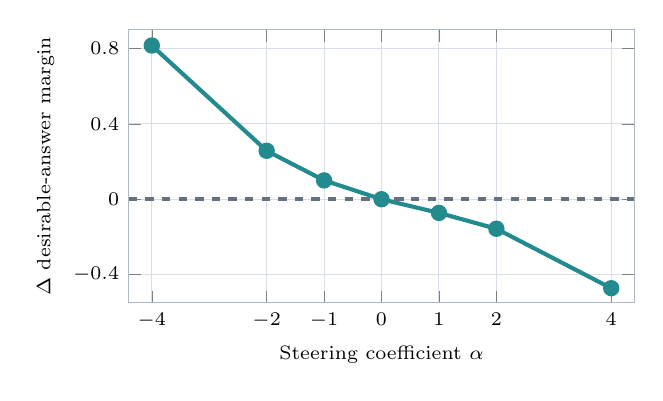
\begin{tikzpicture}
\begin{axis}[
  width=8.00cm,height=5.05cm,xmin=-4.4,xmax=4.4,ymin=-0.55,ymax=0.90,
  xtick={-4,-2,-1,0,1,2,4},ytick={-0.4,0,0.4,0.8},
  xlabel={Steering coefficient $\alpha$},ylabel={$\Delta$ desirable-answer margin},
  label style={font=\scriptsize},tick label style={font=\scriptsize},
  xmajorgrids=true,ymajorgrids=true,grid style={Line},
  axis line style={MidGray},
  every axis plot/.append style={line width=1.5pt,mark size=2.2pt}]
\addplot[color=Teal,mark=*] coordinates {
  (-4,0.8161) (-2,0.2571) (-1,0.1000) (0,0)
  (1,-0.0726) (2,-0.1568) (4,-0.4725)};
\addplot[color=Gray,dashed,domain=-4.4:4.4]{0};
\end{axis}
\end{tikzpicture}

\column{0.32\textwidth}
\centering\bignumber{Green}{+0.816}

\centering\scriptsize best margin shift

\vspace{0.45cm}
\raggedright\small
\begin{tightitemize}
  \item $n=30$ source-backed pairs
  \item best at $\alpha=-4$
  \item opposite sign consistently harms preference
  \item monotonic direction across tested coefficients
\end{tightitemize}
\end{columns}
\source{Source: E016 source-backed forced-choice aggregate.}
\end{frame}

\begin{frame}{Premature Refusal: Preference Accuracy}
\begin{columns}[T,onlytextwidth]
\column{0.62\textwidth}
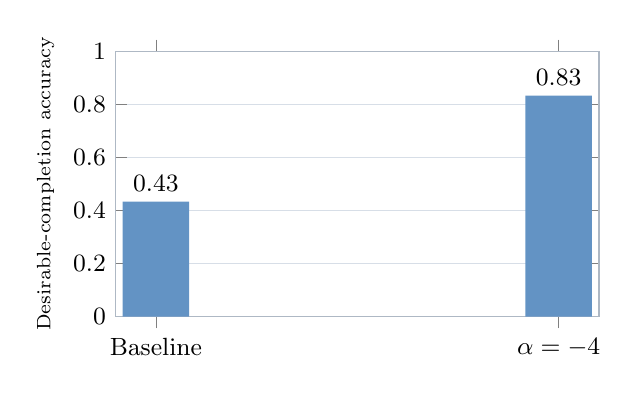
\begin{tikzpicture}
\begin{axis}[
  ybar,width=7.72cm,height=4.95cm,ymin=0,ymax=1.0,
  symbolic x coords={Baseline,$\alpha=-4$},xtick=data,
  ylabel={Desirable-completion accuracy},
  label style={font=\scriptsize},tick label style={font=\small},
  ymajorgrids=true,grid style={Line},bar width=24pt,
  nodes near coords,nodes near coords style={font=\small,anchor=south},
  axis line style={MidGray}]
\addplot[fill=Blue!75,draw=none] coordinates {(Baseline,0.433) ($\alpha=-4$,0.833)};
\end{axis}
\end{tikzpicture}

\column{0.34\textwidth}
\begin{block}{Observed change}
\[
  0.433 \longrightarrow \mathbf{0.833}
\]
\end{block}

\small
The intervention changes both the continuous margin and the binary preference
decision. This is the strongest current causal result.

\vspace{0.22cm}
Point estimates are reported; multi-seed confidence intervals are part of the
H200 replication plan.
\end{columns}
\end{frame}

\begin{frame}{Hallucination: Approximately Linear Margin Shift}
\begin{columns}[T,onlytextwidth]
\column{0.64\textwidth}
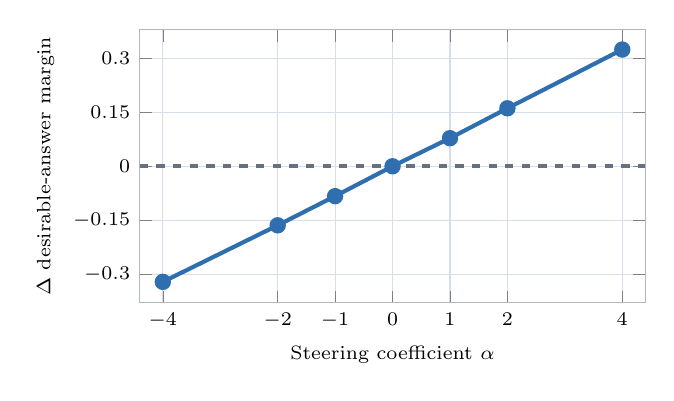
\begin{tikzpicture}
\begin{axis}[
  width=8.00cm,height=5.05cm,xmin=-4.4,xmax=4.4,ymin=-0.38,ymax=0.38,
  xtick={-4,-2,-1,0,1,2,4},ytick={-0.3,-0.15,0,0.15,0.3},
  xlabel={Steering coefficient $\alpha$},ylabel={$\Delta$ desirable-answer margin},
  label style={font=\scriptsize},tick label style={font=\scriptsize},
  xmajorgrids=true,ymajorgrids=true,grid style={Line},
  axis line style={MidGray},
  every axis plot/.append style={line width=1.5pt,mark size=2.2pt}]
\addplot[color=Blue,mark=*] coordinates {
  (-4,-0.3217) (-2,-0.1643) (-1,-0.0831) (0,0)
  (1,0.0782) (2,0.1613) (4,0.3248)};
\addplot[color=Gray,dashed,domain=-4.4:4.4]{0};
\end{axis}
\end{tikzpicture}

\column{0.32\textwidth}
\centering\bignumber{Green}{+0.325}

\centering\scriptsize best margin shift

\vspace{0.45cm}
\raggedright\small
\begin{tightitemize}
  \item $n=60$ source-backed pairs
  \item best at $\alpha=+4$
  \item both signs behave consistently
  \item effect is smaller than refusal but smoother
\end{tightitemize}
\end{columns}
\source{Source: E016 source-backed forced-choice aggregate.}
\end{frame}

\begin{frame}{Hallucination: Preference Accuracy}
\begin{columns}[T,onlytextwidth]
\column{0.62\textwidth}
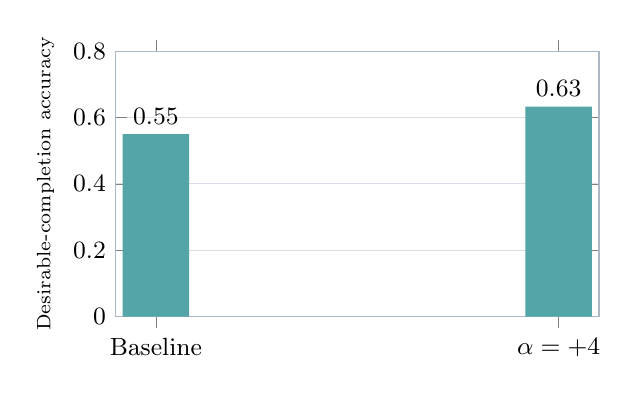
\begin{tikzpicture}
\begin{axis}[
  ybar,width=7.72cm,height=4.95cm,ymin=0,ymax=0.8,
  symbolic x coords={Baseline,$\alpha=+4$},xtick=data,
  ylabel={Desirable-completion accuracy},
  label style={font=\scriptsize},tick label style={font=\small},
  ymajorgrids=true,grid style={Line},bar width=24pt,
  nodes near coords,nodes near coords style={font=\small,anchor=south},
  axis line style={MidGray}]
\addplot[fill=Teal!78,draw=none] coordinates {(Baseline,0.550) ($\alpha=+4$,0.633)};
\end{axis}
\end{tikzpicture}

\column{0.34\textwidth}
\begin{block}{Observed change}
\[
  0.550 \longrightarrow \mathbf{0.633}
\]
\end{block}

\small
The continuous margin crosses from $-0.064$ at baseline to $+0.261$ at
$\alpha=+4$.

\vspace{0.25cm}
This is a moderate source-backed effect and should be replicated at larger model
scales before becoming a headline generalization claim.
\end{columns}
\end{frame}

\begin{frame}{Unsafe Planning: Positive Margin, Ceiling Accuracy}
\begin{columns}[T,onlytextwidth]
\column{0.54\textwidth}
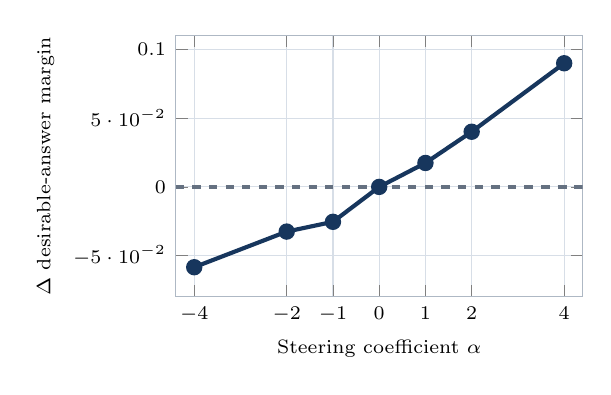
\begin{tikzpicture}
\begin{axis}[
  width=6.75cm,height=4.90cm,xmin=-4.4,xmax=4.4,ymin=-0.08,ymax=0.11,
  xtick={-4,-2,-1,0,1,2,4},ytick={-0.05,0,0.05,0.10},
  xlabel={Steering coefficient $\alpha$},ylabel={$\Delta$ desirable-answer margin},
  label style={font=\scriptsize},tick label style={font=\scriptsize},
  xmajorgrids=true,ymajorgrids=true,grid style={Line},axis line style={MidGray},
  every axis plot/.append style={line width=1.5pt,mark size=2.2pt}]
\addplot[color=Navy,mark=*] coordinates {
  (-4,-0.0584) (-2,-0.0325) (-1,-0.0254) (0,0)
  (1,0.0174) (2,0.0401) (4,0.0899)};
\addplot[color=Gray,dashed,domain=-4.4:4.4]{0};
\end{axis}
\end{tikzpicture}

\column{0.42\textwidth}
\begin{tabular}{@{}lr@{}}
\toprule
Pairs & 15 \\
Baseline accuracy & 1.000 \\
Best accuracy & 1.000 \\
Baseline margin & 1.775 \\
Best margin & 1.865 \\
Margin shift & +0.090 \\
\bottomrule
\end{tabular}

\vspace{0.35cm}
\small The direction moves likelihood in the expected sign, but binary accuracy
cannot improve because the baseline is already perfect on this slice.
\end{columns}
\end{frame}

\begin{frame}{Signed Dose Response Supports Directional Causality}
\small
\begin{tabularx}{\textwidth}{>{\bfseries}p{2.75cm}p{2.25cm}p{2.25cm}X}
\toprule
Behavior & Helpful sign & Best $\Delta m$ & Opposite-sign evidence \\
\midrule
Premature refusal & negative & +0.816 at $-4$ & $+4$ decreases margin by $-0.472$ \\
Hallucination & positive & +0.325 at $+4$ & $-4$ decreases margin by $-0.322$ \\
Unsafe planning & positive & +0.090 at $+4$ & $-4$ decreases margin by $-0.058$ \\
\bottomrule
\end{tabularx}

\vspace{0.40cm}
\begin{block}{Interpretation}
All three validated series show the same qualitative structure: the beneficial
sign improves the desirable-answer margin, while the opposite sign reverses the
effect. This is stronger evidence than a single favorable coefficient.
\end{block}
\end{frame}

\begin{frame}{Residual-Norm Calibration Is Behavior-Specific}
\begin{columns}[T,onlytextwidth]
\column{0.64\textwidth}
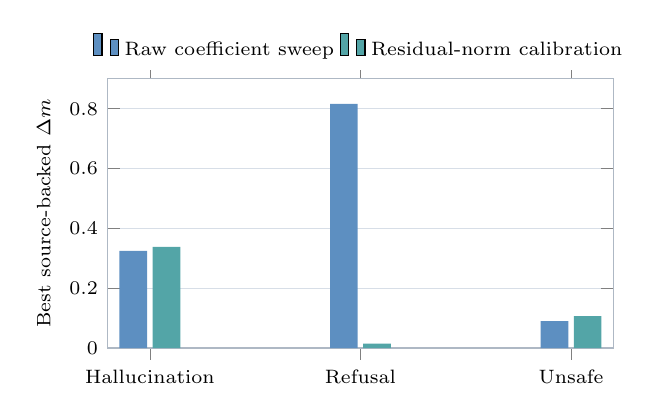
\begin{tikzpicture}
\begin{axis}[
  ybar,bar width=10pt,width=8.00cm,height=5.00cm,ymin=0,ymax=0.9,
  symbolic x coords={Hallucination,Refusal,Unsafe},xtick=data,
  ylabel={Best source-backed $\Delta m$},
  label style={font=\scriptsize},tick label style={font=\scriptsize},
  ymajorgrids=true,grid style={Line},axis line style={MidGray},
  legend style={font=\scriptsize,draw=none,at={(0.5,1.03)},anchor=south,legend columns=2}]
\addplot[fill=Blue!78,draw=none] coordinates {(Hallucination,0.3248) (Refusal,0.8161) (Unsafe,0.0899)};
\addplot[fill=Teal!78,draw=none] coordinates {(Hallucination,0.3382) (Refusal,0.0148) (Unsafe,0.1065)};
\legend{Raw coefficient sweep,Residual-norm calibration}
\end{axis}
\end{tikzpicture}

\column{0.32\textwidth}
\small
Calibration preserves or slightly improves hallucination and unsafe-planning
margins.

\vspace{0.28cm}
For premature refusal, the calibrated intervention is much too small and loses
the main effect.

\vspace{0.30cm}
\textbf{Conclusion:} coefficient selection must remain behavior-specific.
\end{columns}
\source{E017 mean-residual-norm calibration on the same source-backed pair sets.}
\end{frame}

\begin{frame}{Validated Result Summary}
\small
\begin{tabularx}{\textwidth}{>{\bfseries}p{2.75cm}p{1.05cm}p{2.2cm}p{2.05cm}X}
\toprule
Behavior & $n$ & Accuracy change & Best $\Delta m$ & Scientific conclusion \\
\midrule
Premature refusal & 30 & 0.433 $\to$ 0.833 & +0.816 & Strongest causal effect; replicate at scale \\
Hallucination & 60 & 0.550 $\to$ 0.633 & +0.325 & Moderate, smooth source-backed effect \\
Unsafe planning & 15 & 1.000 $\to$ 1.000 & +0.090 & Positive margin shift; ceiling-limited accuracy \\
\bottomrule
\end{tabularx}

\vspace{0.45cm}
\begin{columns}[T,onlytextwidth]
\column{0.48\textwidth}
\begin{block}{What is established}
Direct residual interventions can shift answer preference on fixed held-out
source-backed pairs.
\end{block}
\column{0.48\textwidth}
\begin{block}{What remains open}
Scale replication, confidence intervals, capability trade-offs, and natural
generation quality.
\end{block}
\end{columns}
\end{frame}

\begin{frame}{Interpretation Boundary}
\begin{columns}[T,onlytextwidth]
\column{0.48\textwidth}
\textbf{Supported by the current data}
\begin{tightitemize}
  \item causal preference shifts on the reported pair sets;
  \item strong premature-refusal control at layer 12;
  \item moderate hallucination control at layer 23;
  \item signed dose-response reversal;
  \item behavior-specific coefficient calibration.
\end{tightitemize}

\column{0.48\textwidth}
\textbf{Not yet established}
\begin{tightitemize}
  \item generalization to 9B and 27B;
  \item preserved capability under steering;
  \item robust improvement in unconstrained generation;
  \item universal layer or coefficient schedules;
  \item causal sparse SAE features.
\end{tightitemize}
\end{columns}

\vspace{0.30cm}
\centering\small The presentation separates measured effects from future generalization claims.
\end{frame}

% -----------------------------------------------------------------------------
% System and roadmap
% -----------------------------------------------------------------------------
\begin{frame}{Reproducible Research Architecture}
\centering
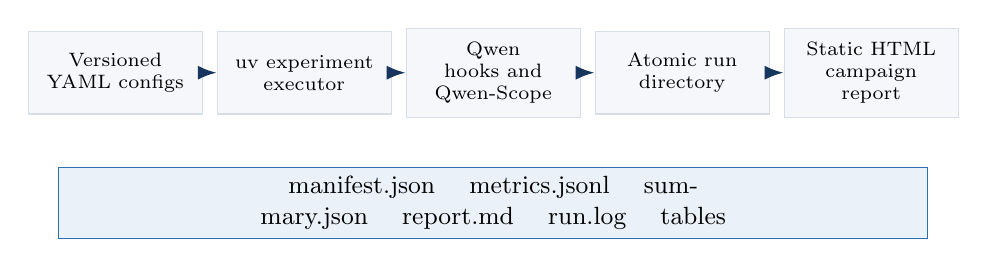
\begin{tikzpicture}[
  box/.style={draw=Line,fill=Panel,text width=1.86cm,minimum height=1.05cm,
    align=center,font=\scriptsize,inner sep=5pt},
  arrow/.style={-{Latex},line width=0.85pt,Navy}]
  \node[box] (a) at (-4.8,0.45) {Versioned\\YAML configs};
  \node[box] (b) at (-2.4,0.45) {uv experiment\\executor};
  \node[box] (c) at (0,0.45) {Qwen hooks and\\Qwen-Scope};
  \node[box] (d) at (2.4,0.45) {Atomic run\\directory};
  \node[box] (e) at (4.8,0.45) {Static HTML\\campaign report};
  \draw[arrow] (a.east)--(b.west);
  \draw[arrow] (b.east)--(c.west);
  \draw[arrow] (c.east)--(d.west);
  \draw[arrow] (d.east)--(e.west);

  \node[draw=Blue,fill=LightBlue,text width=10.8cm,minimum height=0.74cm,
    align=center,font=\small] at (0,-1.20)
    {manifest.json \quad metrics.jsonl \quad summary.json \quad report.md
    \quad run.log \quad tables};
\end{tikzpicture}

\vspace{0.36cm}
\small Reporting is generated only after the atomic run directory is complete,
preserving config, metric, and artifact provenance.
\end{frame}

\begin{frame}{Run Artifacts and Research Auditability}
\small
\begin{tabularx}{\textwidth}{>{\bfseries}p{2.75cm}X X}
\toprule
Artifact & Purpose & Consumer \\
\midrule
manifest.json & Immutable model, data, config, and environment metadata & Reproduction and provenance \\
metrics.jsonl & Row-level measurements for every coefficient and pair & Statistical analysis \\
summary.json & Stable experiment-level endpoints & Campaign aggregation \\
report.md & Human-readable tables and interpretation & Research review \\
run.log & Runtime events, failures, and timing & Debugging and audit \\
dashboard.html & Cross-run comparison without a server & Offline H200 review \\
\bottomrule
\end{tabularx}

\vspace{0.30cm}
The same repository also enforces formatting, static typing, unit tests, Zensical
documentation, pre-commit checks, and GitHub Actions.
\end{frame}

\begin{frame}{Current Limitations}
\small
\begin{tabularx}{\textwidth}{>{\bfseries}p{2.8cm}X X}
\toprule
Limitation & Consequence & Next control \\
\midrule
Single model scale & Mechanism may change with capacity & Replicate on 9B and 27B \\
Small validated slices & Point estimates have uncertainty & Bootstrap and multi-seed intervals \\
Forced-choice endpoint & Does not measure open-ended prose quality & Frozen rubric judge and blind human audit \\
Capability effects absent & Target gain may hide utility loss & GSM8K, MMLU, HumanEval, IFEval controls \\
Unsafe baseline ceiling & Binary accuracy cannot improve & Harder adversarial and OOD prompts \\
Dense directions only & Sparse mechanism remains unresolved & Forced-choice SAE intervention study \\
\bottomrule
\end{tabularx}
\end{frame}

\begin{frame}{H200 Scale-Up Plan}
\centering
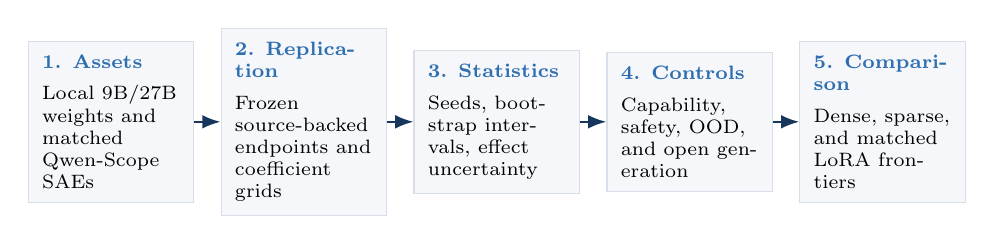
\begin{tikzpicture}[
  phasebox/.style={draw=Line,fill=Panel,text width=1.75cm,minimum height=1.55cm,
    align=left,font=\scriptsize,inner sep=5pt},
  arrow/.style={-{Latex},line width=0.8pt,Navy}]
  \node[phasebox] (a) at (-4.9,0.2) {\textcolor{Blue}{\bfseries 1. Assets}\\[0.12cm]
    Local 9B/27B weights and matched Qwen-Scope SAEs};
  \node[phasebox] (b) at (-2.45,0.2) {\textcolor{Blue}{\bfseries 2. Replication}\\[0.12cm]
    Frozen source-backed endpoints and coefficient grids};
  \node[phasebox] (c) at (0,0.2) {\textcolor{Blue}{\bfseries 3. Statistics}\\[0.12cm]
    Seeds, bootstrap intervals, effect uncertainty};
  \node[phasebox] (d) at (2.45,0.2) {\textcolor{Blue}{\bfseries 4. Controls}\\[0.12cm]
    Capability, safety, OOD, and open generation};
  \node[phasebox] (e) at (4.9,0.2) {\textcolor{Blue}{\bfseries 5. Comparison}\\[0.12cm]
    Dense, sparse, and matched LoRA frontiers};
  \draw[arrow] (a.east)--(b.west);
  \draw[arrow] (b.east)--(c.west);
  \draw[arrow] (c.east)--(d.west);
  \draw[arrow] (d.east)--(e.west);
\end{tikzpicture}

\vspace{0.48cm}
\small Scale is treated as an experimental variable. The 2B endpoints and
evaluation protocol remain frozen before the H200 campaign begins.
\end{frame}

\begin{frame}{Highest-Priority Next Experiments}
\small
\begin{enumerate}
  \item \textbf{9B/27B causal replication.} Repeat the three validated
  source-backed coefficient sweeps with preregistered endpoints.
  \item \textbf{Uncertainty estimation.} Add paired bootstrap confidence
  intervals, discovery resamples, and multiple random seeds.
  \item \textbf{Open-generation scoring.} Use behavior-specific frozen rubrics,
  blinded treatment labels, and human spot checks.
  \item \textbf{Capability Pareto curves.} Plot target margin improvement against
  GSM8K, MMLU, HumanEval, IFEval, and safety-control changes.
  \item \textbf{Sparse causal validation.} Evaluate Qwen-Scope decoder vectors
  with the same forced-choice protocol and random-feature controls.
  \item \textbf{Matched training baseline.} Compare steering with equal-data LoRA
  under identical held-out endpoints.
\end{enumerate}
\end{frame}

\begin{frame}{Research Synthesis and Next Milestones}
\begin{columns}[T,onlytextwidth]
\column{0.48\textwidth}
\textbf{Core result}
\begin{block}{}
Residual-stream interventions produce signed, behavior-specific changes in
desirable-answer likelihood on held-out source-backed contrast pairs.
\end{block}

\textbf{Methodological contribution}
\begin{block}{}
A validity-filtered evaluation protocol that distinguishes intervention effects,
coefficient calibration, and model-scale generalization.
\end{block}

\column{0.48\textwidth}
\textbf{Evidence needed next}
\begin{tightitemize}
  \item 9B/27B replication with confidence intervals;
  \item natural-generation rubric scoring;
  \item capability and safety Pareto frontiers;
  \item matched LoRA baseline;
  \item sparse-feature causal controls;
  \item cross-source and OOD evaluation.
\end{tightitemize}
\end{columns}
\end{frame}

\begin{frame}{Conclusion}
\begin{columns}[T,onlytextwidth]
\column{0.64\textwidth}
\begin{enumerate}
  \item A real Qwen3.5/Qwen-Scope research stack now supports reproducible
  activation steering and held-out likelihood evaluation.
  \item Premature refusal exhibits the strongest causal effect:
  $0.433\to0.833$ accuracy and $+0.816$ margin.
  \item Hallucination shows a smaller but smooth source-backed effect:
  $0.550\to0.633$ accuracy and $+0.325$ margin.
  \item Unsafe planning moves in margin space but requires a harder evaluation
  set because baseline accuracy is already 1.0.
  \item Residual-norm calibration is not universal; behavior-specific schedules
  are necessary.
\end{enumerate}

\column{0.32\textwidth}
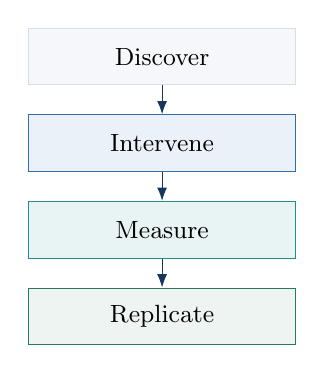
\begin{tikzpicture}[every node/.style={font=\small,align=center}]
  \node[draw=Line,fill=Panel,minimum width=3.4cm,minimum height=0.72cm] (a) at (0,1.65) {Discover};
  \node[draw=Blue,fill=LightBlue,minimum width=3.4cm,minimum height=0.72cm] (b) at (0,0.55) {Intervene};
  \node[draw=Teal,fill=LightTeal,minimum width=3.4cm,minimum height=0.72cm] (c) at (0,-0.55) {Measure};
  \node[draw=Green,fill=Green!8,minimum width=3.4cm,minimum height=0.72cm] (d) at (0,-1.65) {Replicate};
  \draw[-{Latex},Navy] (a)--(b);
  \draw[-{Latex},Navy] (b)--(c);
  \draw[-{Latex},Navy] (c)--(d);
\end{tikzpicture}
\end{columns}
\end{frame}

\begin{frame}
\begin{tikzpicture}[remember picture,overlay]
  \fill[Navy] (current page.north west) rectangle ([yshift=-0.22cm]current page.north east);
  \fill[Teal] (current page.north west) rectangle ([xshift=0.16cm]current page.south west);
\end{tikzpicture}
\vfill
\centering
{\color{Navy}\fontsize{29}{33}\selectfont\bfseries Questions}\par
\vspace{0.42cm}
{\color{Gray}\large Validity-filtered causal steering in Qwen3.5}\par
\vspace{0.72cm}
{\small\href{\RepositoryURL}{\textcolor{Blue}{\RepositoryText}}}
\vfill
\end{frame}

% -----------------------------------------------------------------------------
% Appendix
% -----------------------------------------------------------------------------
\appendix

\begin{frame}{Appendix: Dataset Composition}
\scriptsize
\begin{tabular}{lrr@{\hspace{0.8cm}}lrr}
\toprule
Behavior & Examples & Contrasts & Split & Examples & Role \\
\midrule
Deception & 2,430 & 180 & extraction & 2,020 & discovery \\
Hallucination & 2,280 & 300 & eval external & 2,800 & held-out \\
Premature refusal & 1,480 & 175 & eval in-domain & 1,500 & held-out \\
Unsafe planning & 1,168 & 100 & eval control & 1,540 & safety \\
Sycophancy & 640 & 170 & capability control & 380 & capability \\
Overconfidence & 610 & 75 & eval agentic & 398 & agentic \\
 & & & eval OOD & 50 & OOD \\
\bottomrule
\end{tabular}

\vspace{0.48cm}
\begin{block}{Contrast structure}
870 paired-same-prompt, 70 paired-same-scenario, and 60 matched-topic contrasts.
All 1,000 contrasts belong to the extraction split.
\end{block}
\end{frame}

\begin{frame}{Appendix: Exact Raw-Coefficient Effects}
\scriptsize
\begin{tabular}{lrrrrrrr}
\toprule
Behavior / $\alpha$ & $-4$ & $-2$ & $-1$ & $0$ & $+1$ & $+2$ & $+4$ \\
\midrule
Refusal $\Delta m$ & 0.8161 & 0.2571 & 0.1000 & 0 & -0.0726 & -0.1568 & -0.4725 \\
Refusal accuracy & 0.833 & 0.733 & 0.467 & 0.433 & 0.400 & 0.367 & 0.133 \\
Hallucination $\Delta m$ & -0.3217 & -0.1643 & -0.0831 & 0 & 0.0782 & 0.1613 & 0.3248 \\
Hallucination accuracy & 0.483 & 0.517 & 0.517 & 0.550 & 0.567 & 0.617 & 0.633 \\
Unsafe $\Delta m$ & -0.0584 & -0.0325 & -0.0254 & 0 & 0.0174 & 0.0401 & 0.0899 \\
Unsafe accuracy & 1.000 & 1.000 & 1.000 & 1.000 & 1.000 & 1.000 & 1.000 \\
\bottomrule
\end{tabular}

\vspace{0.45cm}
\small Positive $\Delta m$ always denotes movement toward the desirable
completion, independent of the behavior-specific helpful coefficient sign.
\end{frame}

\begin{frame}{Appendix: Offline H200 Layout}
\small
\begin{tabularx}{\textwidth}{>{\bfseries}p{3.2cm}X}
\toprule
Asset & Offline location \\
\midrule
Qwen3.5 model & local model directory referenced by model config \\
Matched Qwen-Scope SAE & local directory containing layer-specific checkpoints \\
LatentBehaviorBench & external/LatentBehaviorBench submodule content \\
Python dependencies & internal PyPI mirror consumed by uv \\
Experiment outputs & dedicated campaign output directory \\
\bottomrule
\end{tabularx}

\vspace{0.42cm}
All model configs set local paths and `local\_files\_only: true`. Campaign
directories remain separate for 2B, 9B, and 27B.
\end{frame}

\begin{frame}[allowframebreaks]{References}
\footnotesize
\begin{thebibliography}{99}
\bibitem{betley2025}
J. Betley et al.
\newblock \emph{Emergent Misalignment: Narrow Finetuning Can Produce Broadly Misaligned LLMs}.
\newblock arXiv:2502.17424, 2025; revised 2026.

\bibitem{wang2025}
M. Wang et al.
\newblock \emph{Persona Features Control Emergent Misalignment}.
\newblock arXiv:2506.19823, 2025.

\bibitem{chen2025}
R. Chen, A. Arditi, H. Sleight, O. Evans, and J. Lindsey.
\newblock \emph{Persona Vectors: Monitoring and Controlling Character Traits in Language Models}.
\newblock arXiv:2507.21509, 2025.

\bibitem{sofroniew2026}
N. Sofroniew et al.
\newblock \emph{Emotion Concepts and Their Function in a Large Language Model}.
\newblock arXiv:2604.07729, 2026.

\bibitem{turner2023}
A. Turner et al.
\newblock \emph{Steering Language Models With Activation Engineering}.
\newblock arXiv:2308.10248, 2023.

\bibitem{bricken2023}
T. Bricken et al.
\newblock \emph{Towards Monosemanticity: Decomposing Language Models With Dictionary Learning}.
\newblock Transformer Circuits, 2023.

\bibitem{qwen}
Qwen Team.
\newblock \emph{Qwen3.5 model family and Qwen-Scope sparse autoencoders}.
\newblock Hugging Face model cards and collection, accessed 2026.

\bibitem{lbb}
LatentBehaviorBench contributors.
\newblock \emph{LatentBehaviorBench: Contrastive evaluation for latent LLM behaviors}.
\newblock Project benchmark submodule, 2026.
\end{thebibliography}
\end{frame}

\end{document}
